% !TeX root = ../DoABook.tex

\chapter{آنتن‌ها و سیستم دریافت آرایه‌ای}
\label{chap:2}

آنتن در اصل یک مبدل\LTRfootnote{Transducer} است که برای ارسال یا دریافت امواج الکترومغناطیسی یا سیگنال‌های رادیویی که در هوا یا یک محیط منتشر (\lr{propagate}) می‌شوند، طراحی شده است \cite{1}. یک آنتن فرستنده، جریان‌ها را از دستگاه‌های الکترونیکی دریافت کرده و آن‌ها را به سیگنال‌های الکترومغناطیسی یا رادیویی متناظر تبدیل می‌کند که در هوا یا یک محیط تابیده می‌شوند. یک آنتن گیرنده عکس این عمل را انجام می‌دهد: امواج الکترومغناطیسی یا سیگنال‌های رادیویی را در هوا یا یک محیط جذب یا شکار کرده و سپس آن‌ها را به جریان‌های متناظر تبدیل نموده و به دستگاه‌های الکترونیکی متصل ارسال می‌کند. به‌طور خلاصه، آنتن به‌عنوان یک دستگاه واسط\LTRfootnote{Interfacing device} بین هوا (یا یک محیط) و دستگاه‌های الکترونیکی عمل کرده و تحقق یک سیستم بی‌سیم را، همان‌طور که در شکل \ref{fig:2-1} نشان داده شده است، امکان‌پذیر می‌سازد. آنتن‌ها اغلب در سیستم‌هایی مانند پخش رادیویی، مخابرات رادیویی، سیستم‌های تلفن همراه، شبکه‌های محلی بی‌سیم (\lr{LAN})، رادار و کاوش‌های فضایی دیده و استفاده می‌شوند. بدون آنتن‌ها، صنعت مدرن مخابرات بی‌سیم و دورسنجی\LTRfootnote{Telemetry} وجود نداشت.

\begin{figure}[H]
	\centering
	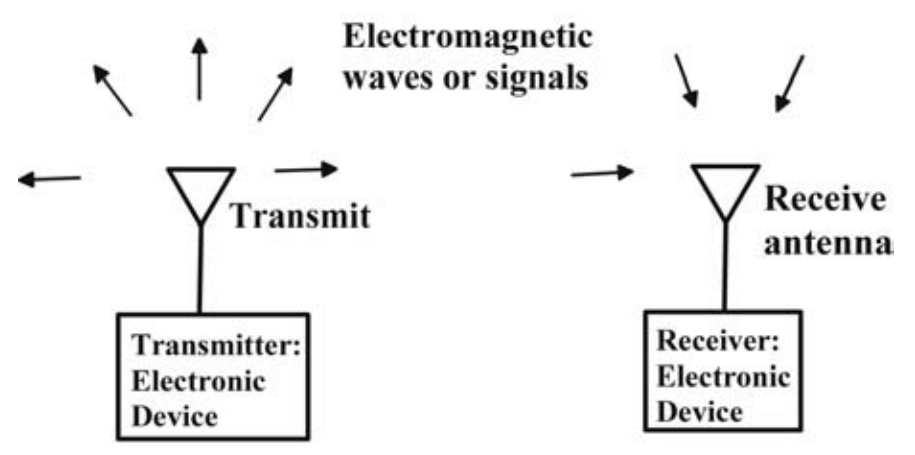
\includegraphics[width=0.6\linewidth]{chapters/figs/fig-2-1}
	\caption{ارسال بی‌سیم از طریق آنتن‌ها.}
	\label{fig:2-1}
\end{figure}




از نظر فیزیکی، یک آنتن آرایشی از رساناها\LTRfootnote{Conductors} و مواد پیرامونی است که در پاسخ به جریان‌ها یا ولتاژهای اعمال‌شده به آن، امواج الکترومغناطیسی تابشی\LTRfootnote{Radiating} تولید می‌کند و یا در اثر تابش\LTRfootnote{impinging} امواج الکترومغناطیسی یا سیگنال‌های رادیویی به آن، جریان‌ها و ولتاژهایی در آن القا می‌شود. روش‌های مختلف آرایش یا قرارگیری رساناها و مواد، منجر به ساخت آنتن‌های متنوعی با رفتارها و ویژگی‌های متفاوت می‌شود. شکل \ref{fig:2-2} یک آنتن تک‌قطبی\LTRfootnote{Monopole antenna} نصب‌شده روی یک خودرو برای دریافت پخش رادیویی و یک آنتن میکرواستریپ پچ\LTRfootnote{Microstrip patch antenna} که در برخی تلفن‌های همراه یا \lr{USB}های بی‌سیم دیده می‌شود را نشان می‌دهد.

\begin{figure}[H]
	\centering
	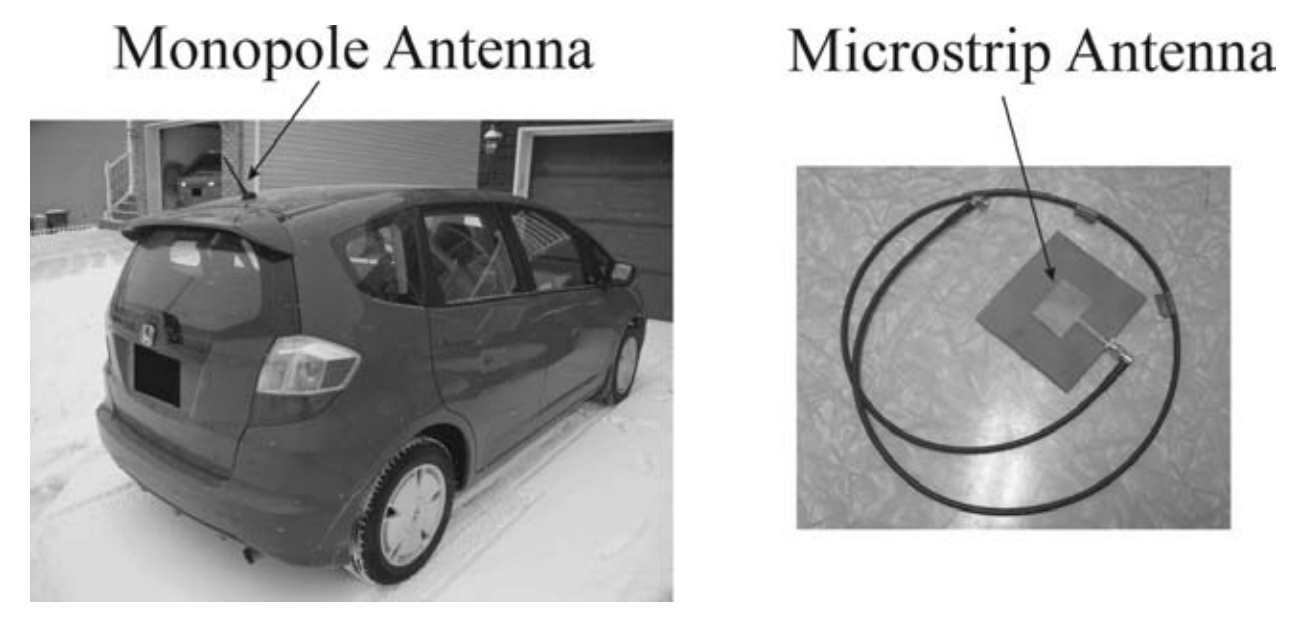
\includegraphics[width=0.7\linewidth]{chapters/figs/fig-2-2}
	\caption{یک آنتن تک‌قطبی نصب‌شده بر روی خودرو و یک آنتن میکرواستریپ پچ.}
	\label{fig:2-2}
\end{figure}

در تئوری، هر دو آنتن فرستنده و گیرنده به دلیل عملکردهای متفاوتشان باید به‌طور جداگانه مطالعه شوند. خوشبختانه، مشخص شده است که توابع فرستندگی و گیرندگی یک آنتن متقابل\LTRfootnote{Reciprocal} هستند. بنابراین، در اکثر متون علمی تاکنون، تنها ویژگی‌های فرستندگی یک آنتن مورد مطالعه و تحلیل قرار گرفته است؛ هنگامی که آنتن برای گیرندگی استفاده می‌شود، ویژگی‌های گیرندگی آن به سادگی و از طریق اصل تقابل\LTRfootnote{Reciprocity} از ویژگی‌های فرستندگی‌اش استخراج می‌شود.

پارامترهای مختلفی برای تعیین کمّی عملکرد یک آنتن معرفی شده‌اند. در این فصل، پارامترها و مفاهیم مهمی را که به تخمین \lr{DOA} مرتبط هستند، شرح خواهیم داد. ابتدا در مورد یک آنتن فرستنده واحد و یک آنتن گیرنده واحد بحث خواهیم کرد و سپس به بررسی آرایه‌های آنتنی\LTRfootnote{Antenna arrays} خواهیم پرداخت که از چندین آنتن واحد تشکیل شده و برای تخمین \lr{DOA} به کار می‌روند.




\section{آنتن فرستنده واحد}
\label{sec:2-1}

یافته‌ها و اثبات‌های علمی نشان می‌دهند که ویژگی‌های زیر برای یک آنتن فرستنده برقرار است:
\begin{enumerate}
	\item انرژی الکترومغناطیسی تابش‌شده از یک آنتن اغلب به‌طور یکنواخت در فضا توزیع نمی‌شود. شدت تابش معمولاً در یک جهت قوی‌تر از سایر جهت‌ها است.
	\item تمامی فرکانس‌های سیگنال‌های رادیویی به‌طور مؤثر از یک آنتن تابش نمی‌شوند. برخی فرکانس‌ها با بازدهی بسیار بالا به هوا یا محیط منتقل می‌شوند و برخی دیگر اصلاً منتقل نمی‌شوند.
\end{enumerate}

برای توصیف این دو پدیده، پارامترهای زیر برای یک آنتن معرفی شده‌اند:
\begin{enumerate}
	\item جهت‌داری\LTRfootnote{Directivity} و بهره\LTRfootnote{Gain} که میزان تمرکز انرژی در یک جهت توسط آنتن را توصیف می‌کنند؛
	\item الگوی تابش\LTRfootnote{Radiation pattern} که شدت‌های تابش نسبی را در تمامی جهت‌ها نشان می‌دهد؛
	\item مدار رزونانس معادل\LTRfootnote{Equivalent resonant circuit} و پهنای باند\LTRfootnote{Bandwidth} که چگونگی رفتار آنتن را از نظر پاسخ‌های فرکانسی نشان می‌دهند.
\end{enumerate}

\subsection{جهت‌داری و بهره}
\label{subsec:2-1-1}

این دو پارامتر اساساً تعیین می‌کنند که یک آنتن تا چه حد می‌تواند انرژی تابشی خود را در یک جهت خاص متمرکز کند. برای این سنجش کمّی، نیاز به یک آنتن مرجع است. در بیشتر موارد، یک آنتن همه‌جهته\LTRfootnote{Omnidirectional antenna} که به‌طور یکسان در تمام جهت‌ها تابش می‌کند، مطابق شکل \ref{fig:2-3} به‌عنوان آنتن مرجع در نظر گرفته می‌شود.

سپس جهت‌داری یک آنتن به‌صورت نسبت شدت توان تابشی آن در یک جهت به شدت توان آنتن همه‌جهته در همان جهت تعریف می‌شود، در حالی که هر دو آنتن توان کل یکسانی را بتابانند. به عبارت دیگر، جهت‌داری یک آنتن میزان شدت توان آن را نسبت به آنتن مرجع (آنتن ایزوتروپیک\LTRfootnote{Isotropic antenna} همه‌جهته) در یک جهت مشخص و در فاصله‌ای دلخواه اندازه‌گیری می‌کند. اگر جهت‌داری در تمام جهت‌ها برابر با یک باشد، آن آنتن یک آنتن همه‌جهته است.

دقیق‌تر آن است که بگوییم جهت‌داری یک آنتن به جهت‌هایی بستگی دارد که شدت تابش در آن‌ها اندازه‌گیری و با آنتن مرجع مقایسه می‌شود. با این حال، در شرایط عادی، واژه جهت‌داری به \textit{بیشینه جهت‌داری} در میان تمامی جهت‌های یک آنتن اشاره دارد.

بهره یک آنتن مستقیماً با جهت‌داری آن در ارتباط است. بهره برابر است با حاصل‌ضرب جهت‌داری در بازده\LTRfootnote{Efficiency} آنتن. بازده، تلفات اهمی توان داخلی آنتن را در نظر می‌گیرد و برابر است با نسبت توان کل تابش‌شده به هوا یا یک محیط توسط آنتن به توان ورودی به آنتن از سوی دستگاه الکترونیکی متصل به آن (شکل \ref{fig:2-4} را ببینید). بازده کمتر یا مساوی $100\%$ است. در نتیجه، بهره همواره کمتر یا مساوی جهت‌داری خواهد بود.

\begin{figure}[ht]
	\centering
	%\includegraphics[width=0.7\textwidth]{fig2-3}
	\caption{آنتن همه‌جهته و توزیع تابش آن.}
	\label{fig:2-3}
\end{figure}






\subsection{الگوی تابش}
\label{subsec:2-1-2}

الگوی تابش یک آنتن، الگوی هندسی از شدت‌های نسبی میدانی است که توسط آنتن با توجه به جهت‌های تابش گسیل می‌شود. برای یک آنتن همه‌جهته ایزوتروپیک ایده‌آل، این الگو یک کره خواهد بود؛ به این معنی که شدت تابش تولیدشده در هر جهت یکسان است. با این حال، برای یک دوقطبی\LTRfootnote{Dipole} معمولی، این الگو به شکل یک چنبره\LTRfootnote{Toroid} یا «دونات» خواهد بود. شکل \ref{fig:2-5} الگوهای دو آنتن، یعنی یک دوقطبی و یک شیپوری موج‌بر\LTRfootnote{Waveguide horn} را نشان می‌دهد. در الگوی تابش، شعاع بلندتر الگو نشان‌دهنده شدت تابش قوی‌تر است. با بررسی الگوی تابش یک آنتن، می‌توانیم مشاهده کنیم که آنتن در کدام جهت بیشترین و در کدام جهت کمترین تابش را دارد.

\begin{figure}[ht]
	\centering
	\caption{الگوهای تابش یک دوقطبی و یک شیپوری موج‌بر (موج‌بر با انتهای باز).}
	\label{fig:2-5}
\end{figure}

\subsection{مدارهای رزونانس معادل و پهنای باند}
\label{subsec:2-1-3}

مانند بسیاری از قطعات مبتنی بر میدان، یک آنتن را می‌توان از نظر ولتاژ و جریان ترمینال ورودی، معادل یک مدار رزونانس در نظر گرفت که در شکل \ref{fig:2-6} نشان داده شده است. در این مدار، علاوه بر مقاومتی که نشان‌دهنده تلفات توان اهمی داخلی آنتن است، مقاومت دیگری به نام مقاومت تابشی\LTRfootnote{Radiation resistor} وجود دارد که میزان توان تابش‌شده به هوا یا محیط را توصیف می‌کند. سلف و خازن نشان‌دهنده ماهیت گزینش‌گر فرکانس\LTRfootnote{Frequency-selective} آنتن هستند. سیگنال‌های ورودی با فرکانس‌های نزدیک به فرکانس رزونانس آنتن می‌توانند به‌راحتی وارد مقاومت تابشی شده و به‌طور معادل، انرژی خود را به هوا یا محیط ارسال کنند.

رابطه معمول بین توان ورودی و فرکانس در شکل \ref{fig:2-7} نشان داده شده است. همانند تعریف پهنای باند برای یک مدار رزونانس، تفاضل بین دو نقطه فرکانسی که در آن‌ها توان به نیمی از مقدار بیشینه خود کاهش می‌یابد، به‌عنوان پهنای باند آنتن تعریف می‌شود. در محدوده پهنای باند، میزان تابش توان را قابل‌قبول در نظر می‌گیریم.

\begin{figure}[ht]
	\centering
	\caption{آنتن و مدار معادل آن.}
	\label{fig:2-6}
\end{figure}

\section{آنتن گیرنده واحد}
\label{sec:2-2}

همان‌طور که پیش‌تر ذکر شد، یک آنتن گیرنده عکس عمل آنتن فرستنده را انجام می‌دهد: انرژی الکترومغناطیسی را در هوا یا محیط جذب و شکار کرده و آن را به جریان‌ها و ولتاژها تبدیل می‌کند. از نظر تئوری، یک آنتن گیرنده نیز باید پارامترهای مخصوص به خود را برای تعیین کمّی عملکردش داشته باشد. به‌ویژه، باید دارای جهت‌داری، بهره و الگوی دریافت مختص به خود باشد که توصیف می‌کنند چگونه یک آنتن گیرنده مقادیر مختلف انرژی سیگنال‌های الکترومغناطیسی یا رادیویی را که از جهت‌های مختلف می‌آیند، در مقایسه با یک آنتن گیرنده همه‌جهته جذب می‌کند. با این حال، مشخص شده است و می‌توان اثبات کرد که این پارامترها دارای مقادیر یا شکلی مشابه با جهت‌داری، بهره و الگوی فرستندگی هستند، مشروط بر اینکه از همان آنتن برای ارسال استفاده شود. در نتیجه، در تقریباً تمامی تحلیل‌های آنتن، جهت‌داری، بهره و الگوی تابش به مواردی ارجاع داده می‌شوند که آنتن برای ارسال استفاده می‌شود. به عبارت دیگر، هنگامی که قرار است از یک آنتن برای دریافت استفاده شود، پارامترهای گیرندگی آن به سادگی از پارامترهای فرستندگی در زمان تحلیل آنتن در حالت ارسال گرفته می‌شوند؛ با این حال، مدار معادل یک استثنا است.

مدار معادل یک آنتن گیرنده در شکل \ref{fig:2-8} نشان داده شده است. این مدار دقیقاً مشابه مدار معادل آنتن در حالت ارسال است، با این تفاوت که یک منبع ولتاژ یا جریان به آن اضافه شده است. منبع جریان نشان‌دهنده جریان معادل القا شده ناشی از حضور میدان‌های الکترومغناطیسی در نزدیکی آنتن گیرنده است. مقاومت‌ها، سلف و خازن مشابه پارامترهای آنتن فرستنده باقی می‌مانند.

\begin{figure}[ht]
	\centering
	\caption{یک رابطه معمول بین فرکانس و توان ورودی به آنتن.}
	\label{fig:2-7}
\end{figure}

\begin{figure}[ht]
	\centering
	%\includegraphics[width=0.7\textwidth]{fig2-8}
	\caption{مدار معادل یک آنتن گیرنده.}
	\label{fig:2-8}
\end{figure}






\section{آرایه آنتنی}
\label{sec:2-3}

آرایه آنتنی\LTRfootnote{Antenna array} گروهی از آنتن‌ها است که برای ارسال یا دریافت سیگنال‌های یکسان استفاده می‌شوند. هر آنتن مجزا اغلب یک عنصر آرایه\LTRfootnote{Array element} نامیده می‌شود. برای یک آرایه گیرنده، سیگنال‌های دریافت شده توسط تمام عناصر آرایه با هم ترکیب شده و سپس برای کاربردهای مختلف، از جمله تخمین \lr{DOA}، پردازش می‌شوند.

به‌منظور تصویرسازی، یک آرایه سه‌عنصری را در نظر بگیرید که به‌طور یکنواخت در امتداد یک خط تراز شده است (شکل \ref{fig:2-9}). راست‌ترین عنصر با شماره $1$ مشخص شده و به‌عنوان عنصر مرجع\LTRfootnote{Reference element} در نظر گرفته می‌شود. دو عنصر دیگر به ترتیب از راست به چپ با شماره‌های $2$ و $3$ نام‌گذاری می‌شوند. فاصله بین دو عنصر مجاور $\Delta$ است. یک منبع امواج الکترومغناطیسی را از چنان فاصله دوری گسیل می‌کند که سه مسیر خطی انتشار از منبع به سه عنصر را می‌توان تقریباً موازی در نظر گرفت. امواج با زاویه $\theta$ به آرایه می‌تابند. در نتیجه، مسیرهای خطی از منبع تا عناصر $2$ و $3$ طولانی‌تر از مسیر تا عنصر $1$ (عنصر مرجع) هستند و این فاصله اضافی برابر است با:
\begin{equation}
	\Delta_m = (m-1) \Delta \sin \theta, \quad m=1, 2, 3
	\label{eq:2-1}
\end{equation}

اکنون فرض کنید سیگنال موج دریافت شده توسط عنصر مرجع (یعنی عنصر $1$)، بدون در نظر گرفتن نویزهای محیط، برابر باشد با:
\begin{equation}
	x_1(t) = s(t)
	\label{eq:2-2}
\end{equation}
در این صورت سیگنال‌های دریافت شده توسط عنصر $2$ و عنصر $3$ را می‌توان به صورت زیر نوشت:
\begin{equation}
	x_2(t) = s(t) e^{-j\beta\Delta_2} = s(t) e^{-j \frac{2\pi}{\lambda} \Delta \sin \theta}
	\label{eq:2-3}
\end{equation}
\begin{equation}
	x_3(t) = s(t) e^{-j\beta\Delta_3} = s(t) e^{-j \frac{2\pi}{\lambda} 2\Delta \sin \theta}
	\label{eq:2-4}
\end{equation}

در اینجا $\beta = 2\pi / \lambda$ ثابت جابجایی فاز\LTRfootnote{Phase shift constant} موج در حال انتشار در هوا و $\lambda$ طول موج است. عبارت جابجایی فاز $e^{-j\beta\Delta_m}$ در روابط \eqref{eq:2-3} و \eqref{eq:2-4}، نتیجه انتشار سیگنال در طول مسیر اضافی $\Delta_m$ در مقایسه با مسیرِ رسیدن به راست‌ترین عنصر است \cite{1}.

در یک حالت کلی‌تر، سیگنال‌های دریافت شده توسط این سه عنصر را می‌توان به صورت زیر نوشت:
\begin{equation}
	\bm{x} = 
	\begin{bmatrix}
		x_1(t) \\
		x_2(t) \\
		x_3(t)
	\end{bmatrix} =
	\begin{bmatrix}
		1 \\
		e^{-j \frac{2\pi}{\lambda} \Delta \sin \theta} \\
		e^{-j \frac{2\pi}{\lambda} 2\Delta \sin \theta}
	\end{bmatrix} s(t) = 
	\begin{bmatrix}
		1 \\
		e^{-j\mu} \\
		e^{-j2\mu}
	\end{bmatrix} s(t) = \bm{a}(\mu) s(t)
	\label{eq:2-5}
\end{equation}
که در آن $\mu = \frac{2\pi}{\lambda} \Delta \sin \theta$ و $\bm{a}(\mu) = [1, e^{-j\mu}, e^{-j2\mu}]^T$ است که اغلب بردار هدایت آرایه\LTRfootnote{Array steering vector} نامیده می‌شود.

معادله \eqref{eq:2-5} قابل تعمیم به یک آرایه $M$-عنصری است و می‌توان آن را به صورت زیر بازنویسی کرد:
\begin{equation}
	\bm{x} = 
	\begin{bmatrix}
		x_1(t) \\
		x_2(t) \\
		\vdots \\
		x_M(t)
	\end{bmatrix} = 
	\begin{bmatrix}
		1 \\
		e^{-j \frac{2\pi}{\lambda} \Delta \sin \theta} \\
		\vdots \\
		e^{-j \frac{2\pi}{\lambda} (M-1)\Delta \sin \theta}
	\end{bmatrix} s(t) = 
	\begin{bmatrix}
		1 \\
		e^{-j\mu} \\
		\vdots \\
		e^{-j(M-1)\mu}
	\end{bmatrix} s(t) = \bm{a}(\mu) s(t)
	\label{eq:2-6}
\end{equation}
و
\begin{equation}
	\bm{a}(\mu) = [1, e^{-j\mu}, \dots, e^{-j(M-1)\mu}]^T
	\nonumber
\end{equation}

اگرچه رابطه \eqref{eq:2-6} برای یک آرایه خطی\LTRfootnote{Linear array} نوشته شده است، اما عبارت $\bm{x} = \bm{a}(\mu)s(t)$ برای هر نوع آرایه دیگری نیز قابل استفاده است.

\begin{figure}[ht]
	\centering
	%\includegraphics[width=0.7\textwidth]{fig2-9}
	\caption{پیکربندی یک آرایه آنتنی سه‌عنصری.}
	\label{fig:2-9}
\end{figure}




\section{نتیجه‌گیری}
\label{sec:2-4}

در این فصل، مفاهیم پایه آنتن‌ها و آرایه‌های آنتنی مرتبط با الگوریتم‌های تخمین \lr{DOA} که در این کتاب مورد بحث قرار می‌گیرند را مرور کردیم. به‌طور خلاصه، آنتن یک دستگاه مبدل است که به منظور ارسال یا دریافت امواج الکترومغناطیسی یا سیگنال‌های رادیویی، میان دستگاه‌های الکترونیکی و هوا (یا یک محیط) واسط می‌شود. این دستگاه می‌تواند ولتاژها/جریان‌ها را به امواج الکترومغناطیسی و بالعکس تبدیل کند. با توجه به این واقعیت که یک آنتن انرژی خود را به‌صورت غیریکنواخت در فضا می‌تاباند، پارامترهایی مانند جهت‌داری، بهره و الگوی تابش اغلب برای تعیین کمّی عملکرد یک آنتن استفاده می‌شوند. از آنجا که آنتن گزینش‌گر فرکانس نیز هست، می‌توان یک مدار معادل را برای توصیف آنتن بر حسب ولتاژ و جریان ترمینال معرفی کرد. به دلیل متقابل بودن عملیات ارسال و دریافت یک آنتن، عملکردهای آنتن اغلب بر اساس ویژگی‌های فرستندگی آن بررسی می‌شوند؛ نتایج حاصل را می‌توان مستقیماً برای ارزیابی عملکرد گیرندگی آن به کار برد.

ادبیات گسترده‌ای در زمینه موضوعات مختلف آنتن منتشر شده است. این حجم عظیم از اطلاعات موجود معمولاً متخصصان حوزه‌های غیرآنتنی را در انتخاب یک متن مناسب به‌عنوان نقطه شروع دچار سردرگمی می‌کند. برای جلوگیری از سردرگمی مشابه، در این فصل تنها به یک مرجع بسنده می‌کنیم. این مرجع، کتاب درسی عالی نوشته‌ی \lr{C. A. Balanis} \cite{1} است؛ این کتاب مقدمه‌ای بر موضوعات مختلف فناوری‌های آنتن، شامل مفاهیم پایه آنتن‌ها و آرایه‌ها را ارائه می‌دهد؛ محتوای این کتاب برای خوانندگان احتمالی اثر حاضر کاملاً کافی است.









